% ============================================================
%  Section — Introduction
% ============================================================

\section{Introduction}
\label{sec:introduction}

The task of entity resolution is to classify the database items (or file records) that refer to the same entity \citep{christen2012data}, where the entity may be person, business, product, etc. In this context, any two items corresponding to the same entity are said to form a \emph{match}, whereas the two items may or may not be classified as a \emph{link} at the result of entity resolution. The need of entity resolution arises in official statistics, machine learning, research or knowledge synthesis, and many other areas, where it is often the prerequisite of downstream tasks that treat the linked dataset as a single source of input. 

Record linkage across two files is a typical problem of entity resolution \citep[e.g.][]{fellegi1969theory, newcombe1959automatic, jaro1989advances, lee2021maximum}. Instead of hand-crafted rules for link classification, the probabilistic approach asks one to model the distortions of the linkage key variables, or simply \emph{keys}, such as (name, date-of-birth, address) for records of persons, so that the decision whether or not to link two records can be largely or entirely data-driven (i.e. without the need for clerical review).

\begin{figure}[ht]
\centering
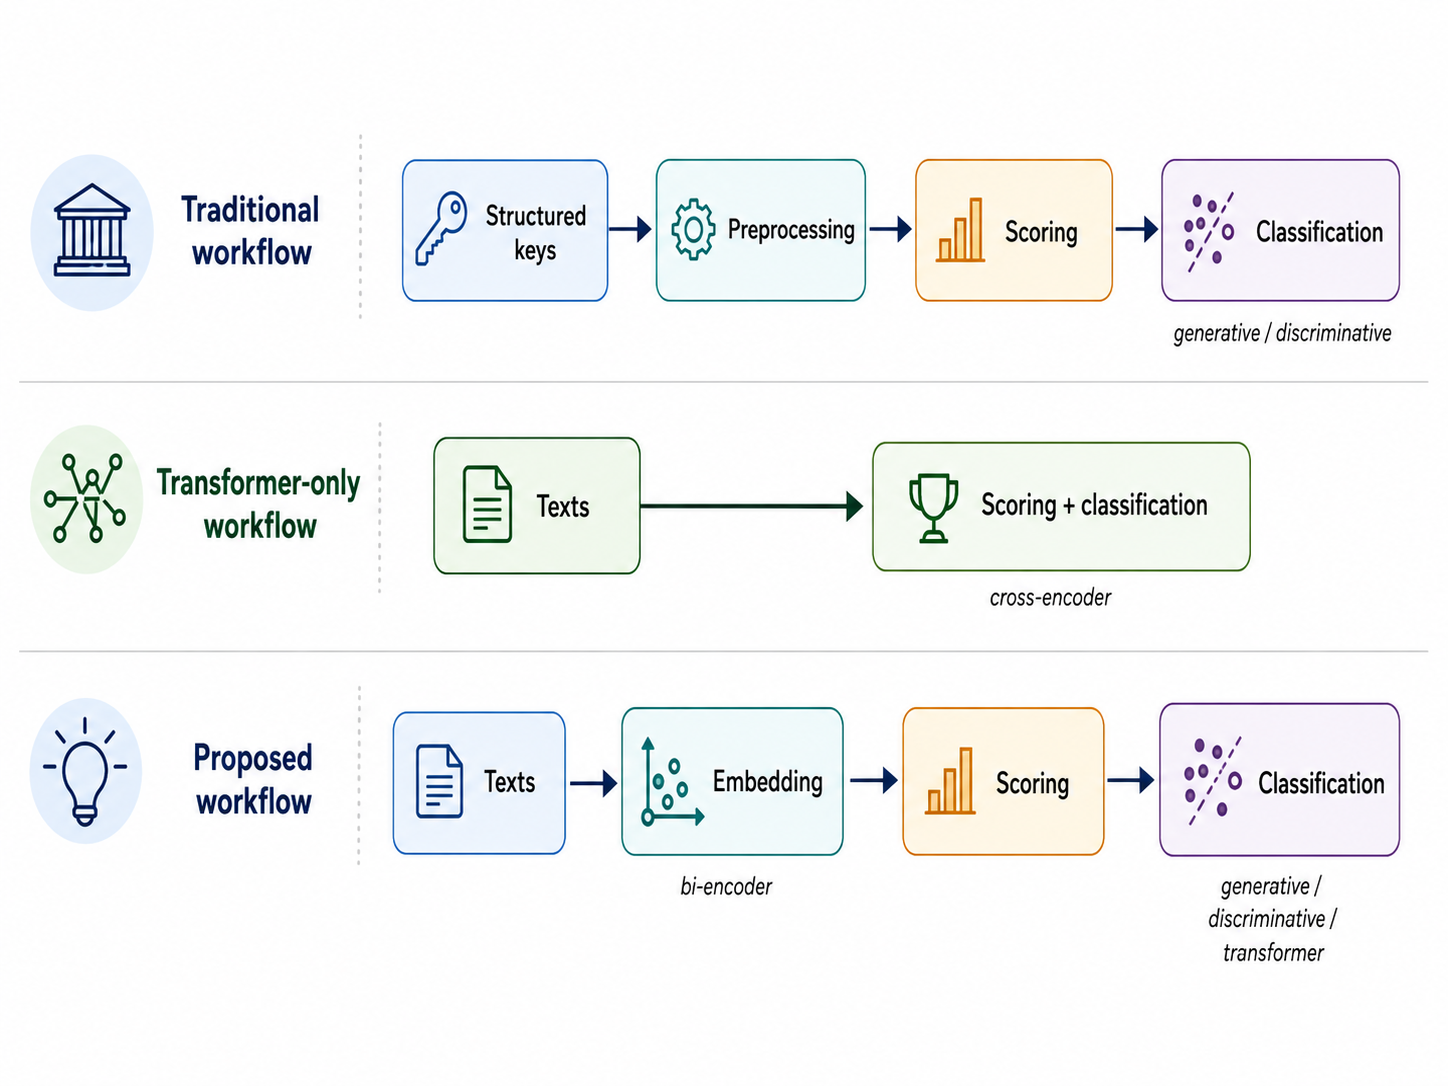
\includegraphics[width=0.85\textwidth]{newsections/images/image_1.png}
\caption{Workflows of entity resolution. Traditional workflow (top), transformer-only workflow (middle), and proposed workflow (bottom).}
\label{fig:workflow}
\end{figure}

The traditional workflow of probabilistic linkage may be given generically as in Figure \ref{fig:workflow}. Although the key values are given as structured data, preprocessing is often necessary to accommodate typical variations of the same key, such as different spellings of an address or name. Scoring then refers to the statistical modelling of the key-value distortions. Two possibilities may be considered.

\begin{itemize}[leftmargin=6mm,itemsep=0pt]

\item Generative models have been common ever since \citet{fellegi1969theory}, where one models the probability of the observed key-value agreement pattern of a pair of records given that they form a match, and the probability given that they do not form a match. The ratio of these two probabilities forms the basis for link classification.

\item Discriminative models target the probability that a pair of records form a match given their observed key values or key-value agreement pattern. While uncommon for record linkage in the unsupervised setting, these models arise naturally in the supervised setting where labelled matches are available. Logistic regression, which we consider later in this paper, is one such model.

\end{itemize}

Finally, \citet{fellegi1969theory} use the likelihood ratio resulting from generative models to classify links and non-links directly, leaving a subset of record pairs to be decided by clerical review. \citet{lee2021maximum} propose maximum entropy classification (MEC) for record linkage based on generative models, which enables fully automated link classification guided by the estimated rates of false links and missing matches.

\begin{table}[ht]
\centering
\caption{Examples of item descriptions in the DBLP-Scholar and Abt-Buy datasets.}
\begin{tabular}{l | l}
\toprule
Field & DBLP-Scholar text \\
\midrule
Title & Distributed Representations of Tuples for Entity Resolution \\
Author & Z Ebraheem, Thirumuruganathan, S. Joty \\
Venue & Proc. VLDB Endow. \\
Year & 2018 \\
\midrule
Field & Abt-Buy text \\
\midrule
Name & Sony Black Pocket AM/FM Walkman Radio - SRF59 \\
Description & Belt Clip Included / Uses 1 AA Battery / Local/DX Switch... \\
\bottomrule
\end{tabular}
\label{tab:text}
\end{table}

However, for entity resolution based on messy texts instead of structured key values, it is often difficult and ineffective to formulate deterministic rules of preprocessing. Table \ref{tab:text} gives two examples, one from the DBLP-Scholar dataset and the other from the Abt-Buy dataset, both in the Magellan data repository of benchmark datasets for entity resolution \citep{konda2016magellan}; see Appendix \ref{app:datasets} for details.

The text data in DBLP-Scholar are structured in four fields. Although the content can be quite noisy for some fields, such as author names, one might still attempt preprocessing of these texts by hand-crafted rules. In contrast, the relatively free-form texts in the Abt-Buy dataset may be highly irregular from one product to another, and it is not obvious that traditional preprocessing rules for keys such as name and address would be effective for the product names and descriptions here.

It is therefore natural to consider machine learning models that can work directly with such text. \citet{mudgal2018deep} show that deep-learning models can outperform hand-crafted feature engineering for text-based entity resolution. More recently, transformer models, introduced by \citet{vaswani2017attention}, have provided a way to represent and compare texts while taking their context into account. The transformer architecture uses self-attention to model relationships between tokens within a sequence, which makes it particularly suitable for handling textual data.

In the work of \citet{li2020deep}, entity resolution is cast as a sequence-pair classification task using a pretrained transformer language model. The two records are supplied jointly to the model, allowing the self-attention layers to represent interactions across the paired input. This type of architecture is commonly referred to as a \emph{cross-encoder}.

The computational cost becomes prohibitive, however, if the cross-encoder is applied to every possible pair of records, as we shall illustrate later using the DBLP-Scholar and Abt-Buy datasets. A \emph{bi-encoder} transformer model \citep{reimers2019sentence, wang2022sudowoodo} instead encodes each text separately as a numerical vector, or \emph{embedding}. Similarity between these embeddings can then be used to identify a much smaller set of candidate records before more expensive scoring or classification is applied. This provides a form of semantic blocking, analogous to traditional blocking in record linkage. For instance, \citet{reimers2019sentence} report that finding the most similar pair in a collection of $10{,}000$ sentences required about 65 hours with a standard BERT model, compared with about 5 seconds using SBERT embeddings and cosine similarity.

Bi-encoder blocking greatly reduces the number of record pairs that require further comparison, but it still leaves several choices about how the candidate pairs should be scored and classified. In particular, the numerical representations produced by a bi-encoder can be combined with traditional generative or discriminative scoring methods, or the candidate texts can be passed to a cross-encoder for classification. The usefulness of these alternatives may also change after the transformer models are fine-tuned to the texts of a particular application. These considerations motivate the integrated workflow in Figure \ref{fig:workflow}, as well as a closer examination of the linkage errors associated with the resulting models.


\subsection{Proposed workflow using transformer models}
\label{sec:proposal}

Our proposed workflow for entity resolution is given in Figure \ref{fig:workflow}, which uses transformer models as well as traditional generative or discriminative models.

While the workflow is applicable to both the supervised and unsupervised settings, i.e. with or without a sample of labelled matches, we shall focus on the supervised setting in this paper. Transformer models are considered for embedding and classification. Notice that cross-encoder models with text as input are not relevant for scoring given numerical embeddings, whereas how to use transformer models to achieve scoring-classification from texts directly remains an open question in the unsupervised setting.

A fundamental difficulty for modelling arises from the following fact about entity resolution. While matched items refer to real entities, a pair of non-matches does not correspond to a single real entity. For instance, when two records refer to two different persons, there is no person associated with both records. It follows that there is no naturally defined population of non-matches corresponding to the population of matches, which complicates the construction of training data for supervised learning.

To deal with this difficulty, it is common to create the training and test sets in a way that
mirrors how the models will later be applied to out-of-sample items. Suppose that, for each
out-of-sample record in $A$, one would conduct blocking to gather $k$ candidate records in
$B$ for scoring and classification. We then construct candidate records in the same manner
for the sampled file-$A$ records, and partition those file-$A$ records into training and test
sets together with their associated candidate records. Thus, all candidate pairs associated
with a given file-$A$ record remain in the same partition. Duplication of candidate records
for different records in $A$ is allowed if it is also allowed for the out-of-sample records in
application.

Notice that, if none of the valid matched records is selected among the $k$
candidates, the corresponding file-$A$ record cannot be linked correctly. Hence the
choice of $k$ induces a floor of missing match rate (MMR). In practice, for scoring
and classification, it is natural to select the $k$ most likely link candidates for
blocking, i.e. the records in $B$ with the most similar texts, and to choose $k$ such
that the MMR floor is considered acceptable. Selecting the most similar candidates
also provides more difficult non-matches for supervised learning than selecting
non-matches randomly.

In addition to the MMR, another central performance measure is the \emph{false linkage rate (FLR)}. We use the FLR and MMR, following the definitions of \citet{lee2021maximum}, for the evaluation and comparison of the different methods considered in this paper. Their formal definitions in the present setup are given in Section \ref{sec:setting}. Notice that both are well-defined whether or not one employs additional treatments of duplicated candidate records for scoring and classification.

The details of the steps in the proposed workflow will be studied in this paper, and the relevant methodological choices exemplified and compared.


 

\subsection{Link classification errors by transformer models}
\label{sec:literature:error}

The estimation of FLR and MMR for link classification based on transformer models requires special attention.

\rev{If one uses only a pretrained transformer model that is fixed independently of the labelled data, then, under the SRSWOR assumption stated in Section~\ref{sec:setting}, the observed errors in the labelled file-$A$ sample may be used to estimate the FLR and MMR that would arise over the corresponding finite population of file-$A$ records. This population interpretation is conditional on the labelled records being a probability sample from that population. In the benchmark experiments below, by contrast, the available benchmark data are partitioned internally into training and test sets. The resulting FLR and MMR are therefore internal test-set quantities; they should not be interpreted directly as design-based estimates for a wider operational database unless the stated sampling assumption holds.}

The matter becomes more complicated when the transformer model is fine-tuned using the labelled sample. An obvious approach is to split the labelled sample into a training set for fine-tuning and a test set for estimating the errors of the resulting subsample-tuned model. This is valid if one is willing to apply that subsample-tuned model directly to the out-of-sample items. It is not sufficient, however, if the subsample training is used only to determine the hyperparameters of fine-tuning, after which the transformer model is fine-tuned again using the entire labelled sample and this final model is applied to the remaining records. The errors observed on the original test set then refer to a different fitted model from the one eventually used for entity resolution.

We shall study this issue later using the DBLP-Scholar and Abt-Buy datasets, illustrating both the statistical problem and the practical difficulties that arise. Below we briefly explain why the issue also presents difficulties for several existing approaches to error assessment.

\emph{Bayesian uncertainty propagation.}
In Bayesian approaches to entity resolution, one may model the key values or their disagreement patterns and generate link sets according to the posterior distribution of the matches, conditional on the observed keys; see, for example, \citet{tancredi2011hierarchical, sadinle2017bayesian, steorts2016bayesian}. It is unclear how such prior-posterior uncertainty propagation can be carried through a fine-tuned transformer model, which does not provide the likelihood function required for the corresponding Bayesian calculation. Moreover, repeatedly generating link sets while refitting or evaluating a large transformer model would be computationally expensive.

\emph{Auditing.}
A practical approach in the unsupervised setting of entity resolution is to draw an audit sample from the classified links in order to estimate the FLR \citep{christen2012data}; see also \citet{binette2024evaluation} for a more elaborate proposal. In the supervised setting, the labelled match sample can be used to estimate both FLR and MMR when the classification model is fixed independently of that sample. The situation changes when the same labelled observations are used for fine-tuning. Auditing additional out-of-sample records could provide information about the final model, but identifying their true matches may require substantial clerical effort.

\emph{Design-based sample inference.}
\citet{zhang2025predictive, zhang2026debiasing} develop unbiased estimation of algorithmic prediction or classification errors under finite population sampling. In principle, this provides a way to accommodate models trained using sampled observations. In practice, however, the required calculations can be costly for transformer models. Moreover, although link classification can be viewed as a special case of classification, unbiased estimation of classification errors in this framework relies on randomised prediction or classification, whereas deterministic classification is generally preferred for record linkage.




\subsection{Notations and rest of paper}
\label{sec:setting}

Let us now introduce the basic notations related to the workflow of entity resolution, formalising the concepts discussed above and preparing for the investigations later.

Without loss of generality, let us use the standard setup of record linkage across two files. Let
$A = \{a_1, \ldots, a_{n_A}\}$ and
$B = \{b_1, \ldots, b_{n_B}\}$
be two files containing $n_A$ and $n_B$ records, respectively. Let entity resolution, or record linkage, be based on
$\{\tau_i : i \in A \cup B\}$,
where $\tau_i$ is the text associated with record $i$, which may or may not consist of structured fields, as exemplified in Table \ref{tab:text}.

Let $M$ be the set of matches, $M \subset A \times B$, and denote a match by $(i,j) \in M$, or equivalently $y_{ij}=1$, if records $i$ and $j$ refer to the same entity. A non-match is denoted by $(i,j) \notin M$, or $y_{ij}=0$. Let $A(M)$ and $B(M)$ denote the records in $A$ and $B$, respectively, belonging to $M$.

Let $A_s\subseteq A$ denote the sampled file-$A$ records. For simplicity of
exposition in this paper, we assume that $A_s$ is obtained from $A$ by simple random
sampling without replacement (SRSWOR). Let

\[
s_M=\{(i,j)\in M:i\in A_s\}
\]

denote the labelled match relation induced by these sampled records. Let $A(s_M)$
denote the records in $A_s$ having at least one match in $s_M$, and let $B(s_M)$
denote the corresponding matched records in $B$. Thus,
$A_s\setminus A(s_M)$ contains the sampled file-$A$ records that are non-matchable.

In practice, one first draws the file-$A$ records in $A_s$ and then identifies all
their known matches by any means necessary. This formulation samples file-$A$
records rather than individual matched pairs. The distinction becomes relevant when
a file-$A$ record has more than one valid partner in $B$.

To limit the number of comparisons for the models, let $C_i$ denote the block of candidate records for each $i \in A$ according to a given blocking scheme, where
$C_i \subset B$, and $C_i \cap C_j$ may be non-empty for $i \neq j \in A$. Let $k$ be the size of $C_i$ in the case $|C_i| \equiv k$.

By applying a \emph{given} model of link classification to
\[
\{(i,j) : i \in A_s,\; j \in C_i\},
\]
denote by $\ell_i=1$ if $i \in A_s$ is linked and $\ell_i=0$ if it is not linked. One can estimate the FLR and MMR when the model is applied to all the record pairs
\[
\{(i,j) : i \in A,\; j \in C_i\},
\]
as
\begin{equation}
\label{eq:FLR:MMR}
\widehat{\mathrm{FLR}}
=
1-
\frac{
\sum_{i \in A(s_M)} \ell_i y_{ij_i}
}{
\sum_{i \in A_s} \ell_i
},
\qquad
\widehat{\mathrm{MMR}}
=
1-
\frac{
\sum_{i \in A(s_M)} \ell_i y_{ij_i}
}{
|A(s_M)|
},
\end{equation}
where $j_i$ refers to the linked record in $B$ given $\ell_i=1$, and
$y_{ij_i} \equiv 0$ if $i \in A \setminus A(M)$.

For supervised learning including non-matches in addition to matches, let
$(A_1,A_2)$ denote a partition of $A_s$, where

\[
A_1\cup A_2=A_s,
\qquad
A_1\cap A_2=\emptyset.
\]

We use $A_1$ for training and $A_2$ for testing. Let

\[
s_r=\{(i,j)\in s_M:i\in A_r\},
\qquad r=1,2,
\]

denote the labelled match relations induced by these two sets of file-$A$ records.
Thus, all known matches belonging to the same file-$A$ record remain on the same
side of the training-test partition.

According to the setup in Section 1.1, the corresponding candidate non-matches
associated with matchable records are

\[
\bigcup_{i\in A_1\cap A(s_M)}
\{(i,j):j\in C_i,\ y_{ij}=0\}
\]

for training and

\[
\bigcup_{i\in A_2\cap A(s_M)}
\{(i,j):j\in C_i,\ y_{ij}=0\}
\]

for testing. For non-matchable sampled file-$A$ records, all candidate pairs are
non-matches, giving

\[
\bigcup_{i\in A_r\setminus A(s_M)}
\{(i,j):j\in C_i\},
\qquad r=1,2.
\]

Notice that the setup of supervised learning above can vary with the blocking scheme. In particular, given the fixed block size $k$, we consider two schemes.

\begin{itemize}[leftmargin=2mm,itemsep=0pt]

\item[] \emph{Scheme-I}: for each $i \in A(s_M)$, let $C_i$ contain one retained matched record $j$ for which $(i,j) \in s_M$, together with $k-1$ non-matches.

\item[] \emph{Scheme-II}: for each $i \in A(s_M)$, let $C_i$ consist of the $k$ most similar file-$B$ records.

\end{itemize}

Under Scheme-I, the retained labelled match is inserted into each candidate block, whereas under
Scheme-II the candidate block is determined entirely by similarity and may therefore fail
to contain a valid match. The difference between the two schemes decreases as the block
size $k$ increases. Scheme-I makes more efficient use of the labelled matches for learning,
while Scheme-II is more closely related to the application of the models to out-of-sample
records.

In the experiments below we use Scheme-II to construct the candidate blocks. For supervised
fitting, however, one known valid file-$B$ partner is retained as the positive example for each
matchable file-$A$ record, whether or not that particular retained partner occurs in $C_i$.
The non-match examples are drawn from $C_i$, with every known valid partner excluded from
the non-match class. At evaluation, $C_i$ is not augmented in this way: a predicted link must
be selected from the retrieved candidate block, and failure to retrieve any valid partner
contributes to the floor MMR.

Section \ref{sec:experimental-setup} describes the datasets and experimental setup used throughout the empirical analysis. We study the proposed workflow using pretrained transformer models in Section \ref{sec:pretrained}. Section \ref{sec:finetuning} considers the fine-tuning of transformer models, including the related assessment of link classification errors. Section \ref{sec:final-remarks} provides the final remarks and discusses topics for future research and development.

